
\chapter{交通信号灯控制方法}
\label{ch4}
本章将要介绍降低道路饱和度信号控制方法、信号抢占方法、恢复交通流方法。

%由于一个交叉口可能受到单个应急车辆或者多个应急车辆的请求,本文针对不同情况设计了面向单个应急车辆的降低道路饱和度方法和面向多辆应急车辆的降低道路饱和度方法。信号抢占方法包含了非侵入式信号抢占方法和侵入式信号抢占方法。


%本小结将要介绍降低道路饱和度的目的和降低道路饱和度需求度计算模型。由于一个交叉口可能受到单个应急车辆或者多个应急车辆的请求,本文针对不同情况设计了面向单个应急车辆的降低道路饱和度方法和面向多辆应急车辆的降低道路饱和度方法。

\section{按需降低道路饱和度及普通车辆让行}
\subsection{降低道路饱和度的目的}
为了使得应急车辆在道路上行驶的过程中受普通车辆的影响尽可能小,本文通过降低道路饱和度的方式使得普通车辆有空间为应急车辆让行,如图\ref{fig:highsituration}所示,当道路饱和度较高时,普通车辆无法为应急车辆让行,因此普通车辆限制了应急车辆的行驶,使得应急车辆无法以更快的速度行驶,进而间接性地延长了应急车辆的旅行时间。
\begin{figure}[ht]
	\centering
	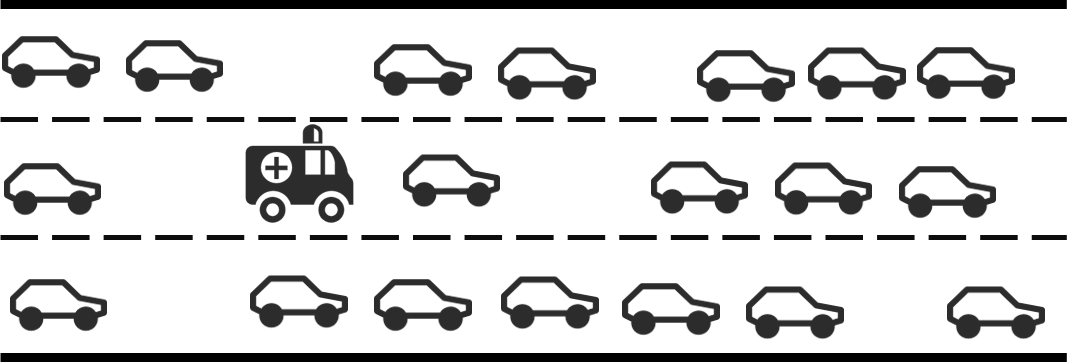
\includegraphics[width=\textwidth]{figures/highsituration.png}
	\caption{道路饱和度较高,普通车辆无法让行}
	\label{fig:highsituration}
\end{figure}

本文希望通过降低饱和度,使得应急车辆有空间为应急车辆让行,如图\ref{fig:lowsituration}所示,道路饱和度相对较低,普通车辆向道路两旁让行,应急车辆前方无其他车辆,这为应急车辆创造了卓越的道路条件,因此应急车辆可以以更快地速度行驶,进而缩短旅行时间。

\begin{figure}[ht]
	\centering
	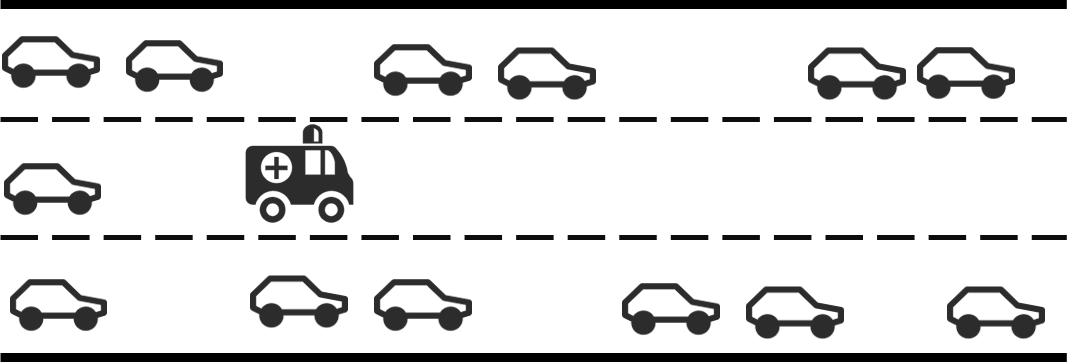
\includegraphics[width=\textwidth]{figures/lowsituration.png}
	\caption{道路饱和度降低,普通车辆让行}
	\label{fig:lowsituration}
\end{figure}

在交叉口层面,当道路饱和度较高时,交叉口在应急车辆前进方向的入口道上聚集了大量的社会车辆。本文希望在应急车辆到达交叉口之前,尽量减少应急车辆入口车道的排队车辆数,并且在应急车辆通过路口后,前方的排队车辆也可以及时地给紧急车辆让行,这将体现在下一节的信号抢占部分。

为了更好地解释降低道路饱和度在交叉口层面的作用,用图\ref{fig:tl_unreduce}和\ref{fig:tl_unreduce_passed}表示没有使用降低道路饱和度信号控制算法,应急车辆在到达交叉口之前与到达交叉口时入口车道上的交通情况。图\ref{fig:tl_reduce}和\ref{fig:tl_reduce_passed}表示使用降低道路饱和度信号控制算法,应急车辆在到达交叉口之前与到达交叉口时入口车道上的交通情况。图中仅画出应急车辆所在车道的车辆,其余车辆暂不考虑。


图\ref{fig:tl_unreduce}表示在不实施降低道路光饱和度信号控制算法的情形下,由于应急车到达路口时的前面排队车辆较多,因此必须等到前面的排队车辆全部清空后方可通过路口。图\ref{fig:tl_unreduce_passed}的情况下,应急车辆通过交叉口后,前方有普通车辆阻碍了应急车辆的前进,使得应急车辆无法以更快的速度行驶。

\begin{figure}[H]
	\centering
	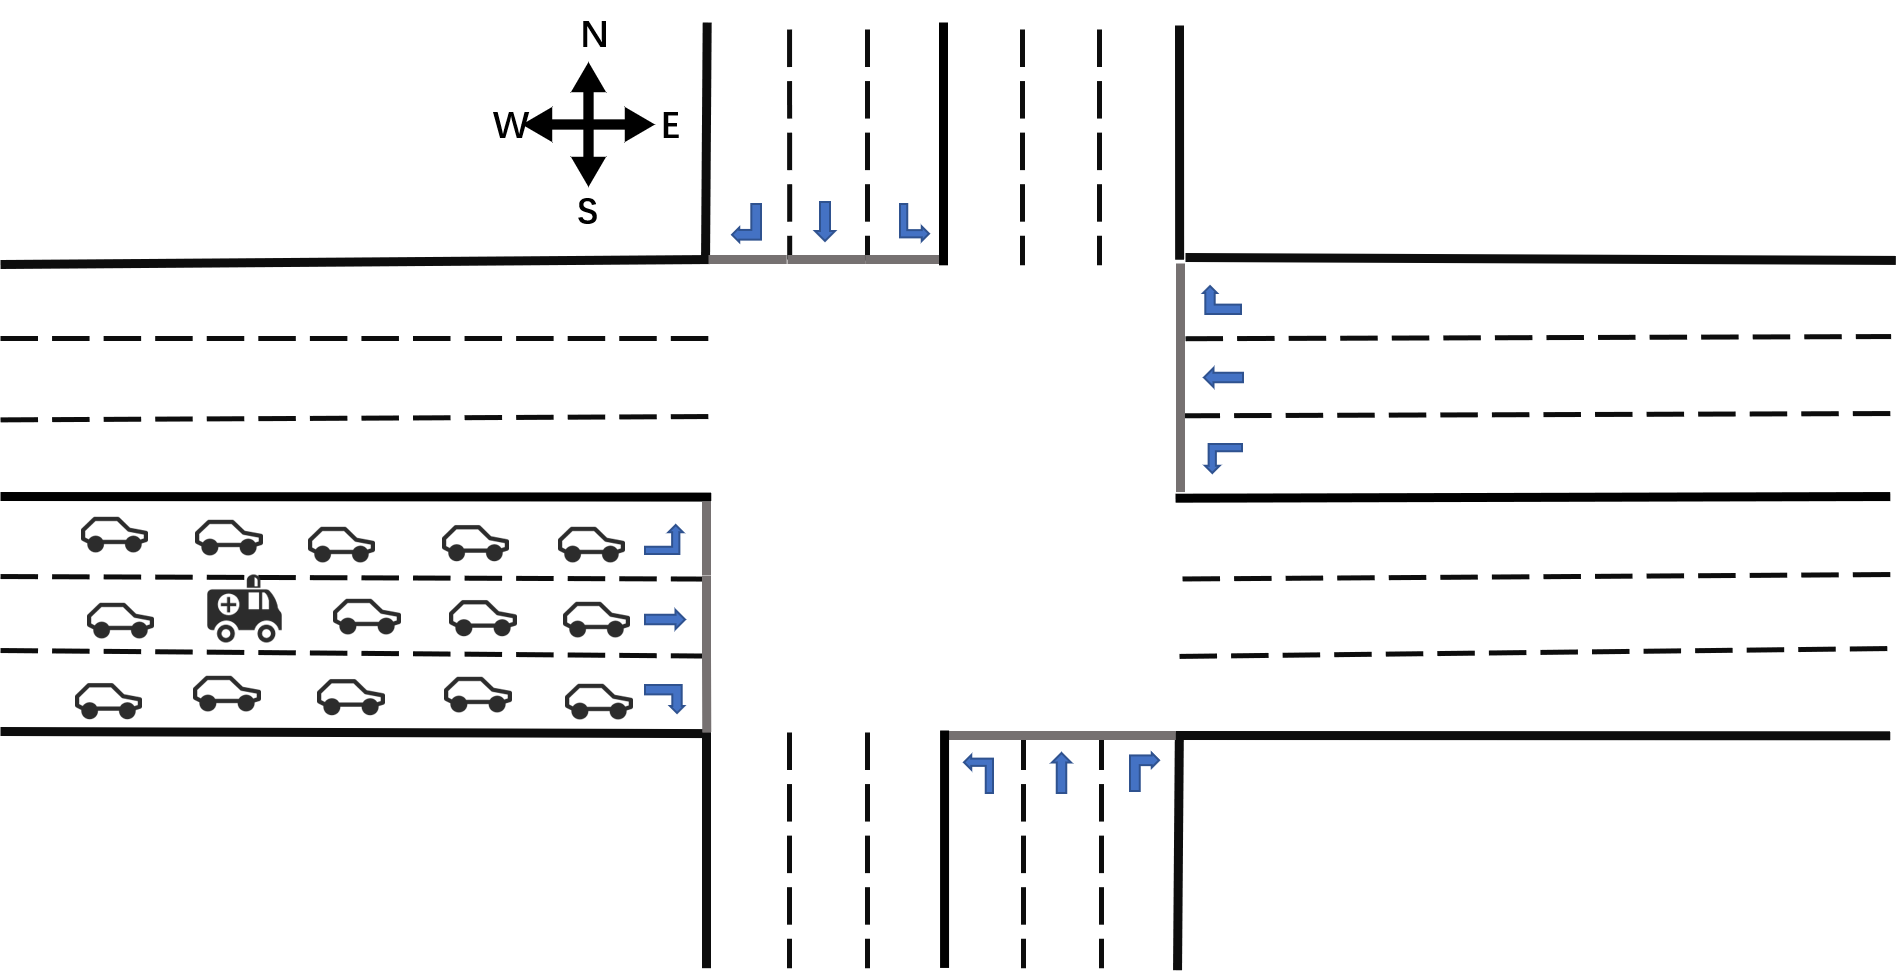
\includegraphics[width=\textwidth]{figures/tl_unreduce.png}
	\caption{不采取降低道路饱和度信号控制算法,应急车辆到达交叉口时道路情形图}
	\label{fig:tl_unreduce}
\end{figure}

\begin{figure}[H]
	\centering
	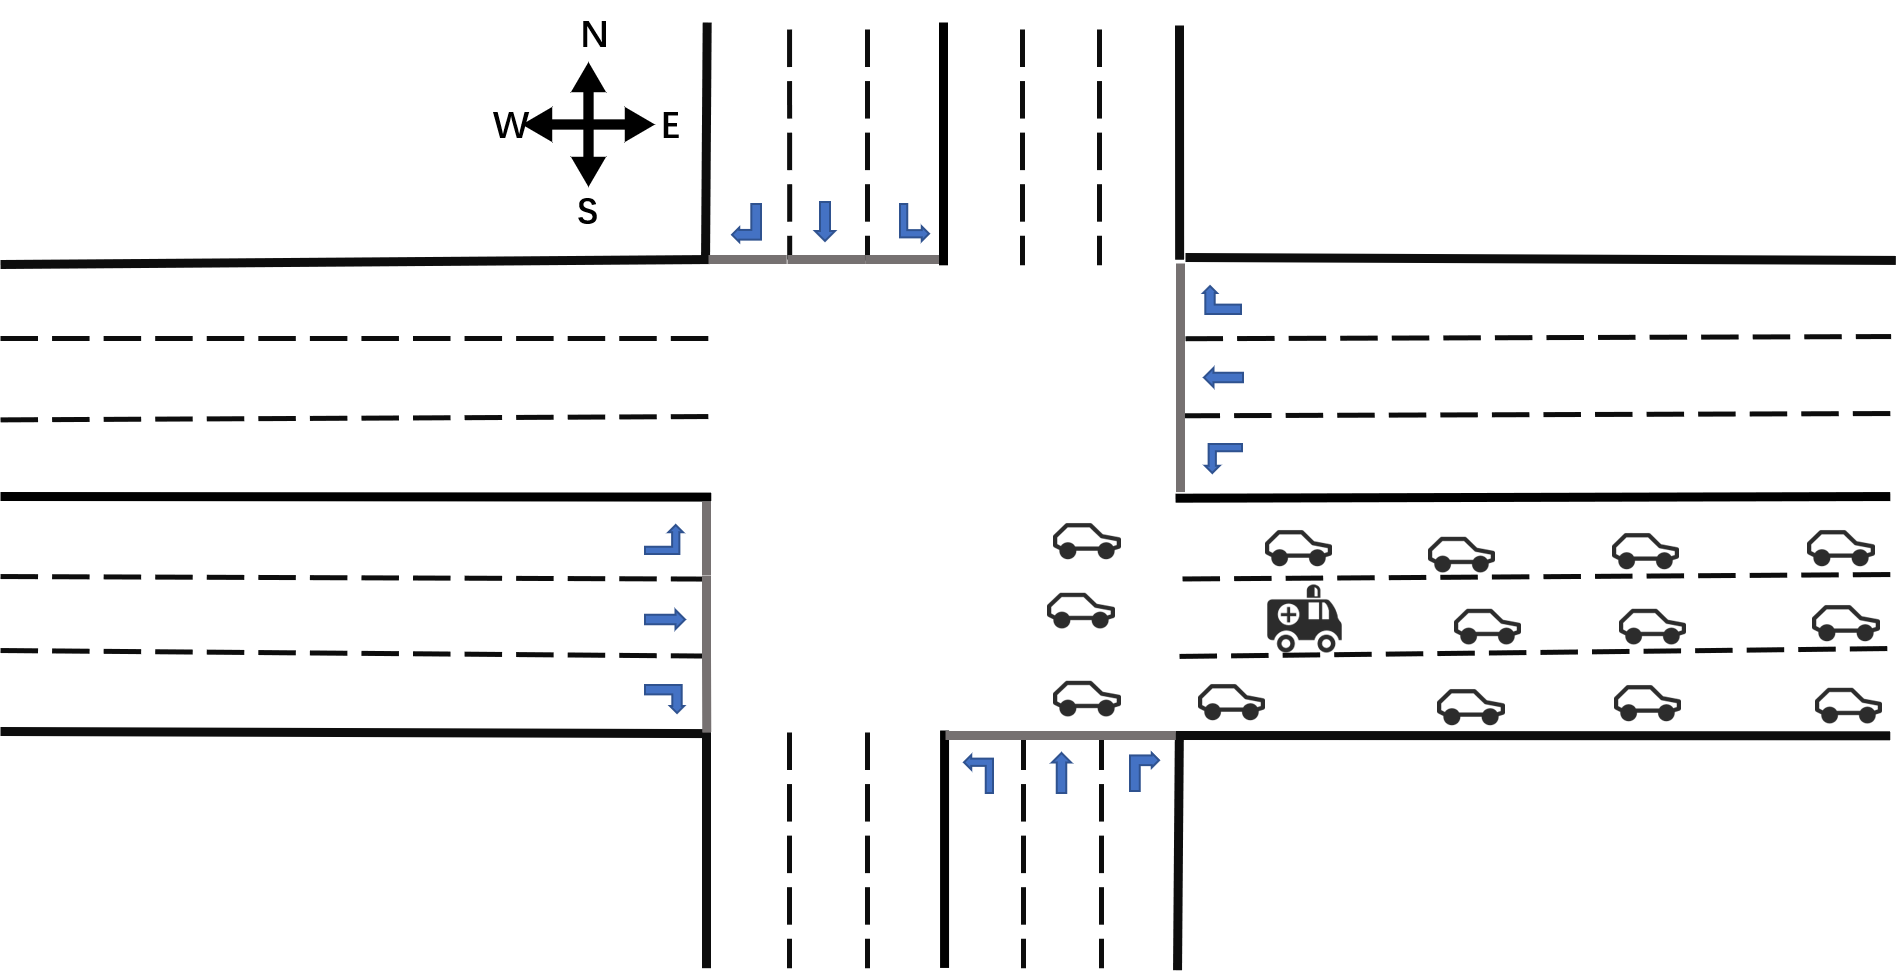
\includegraphics[width=\textwidth]{figures/tl_unreduce_passed.png}
	\caption{不采取降低道路饱和度信号控制算法,应急车辆通过交叉口后道路情形图}
	\label{fig:tl_unreduce_passed}
\end{figure}

图\ref{fig:tl_reduce}表示在采取降低道路饱和度信号控制算法的情况下,应急车辆到达交叉口时的前方排队车辆与图\ref{fig:tl_unreduce_passed}相对减少,需要等待前方排队车辆清空的时间也会相对地减少。图\ref{fig:tl_reduce_passed}表示在采取降低道路饱和度信号控制算法的情况下,应急车辆通过交叉口后,前方没有普通车辆阻碍应急车辆的前进,使得应急车辆能够以更快的速度行驶。


\begin{figure}[H]
	\centering
	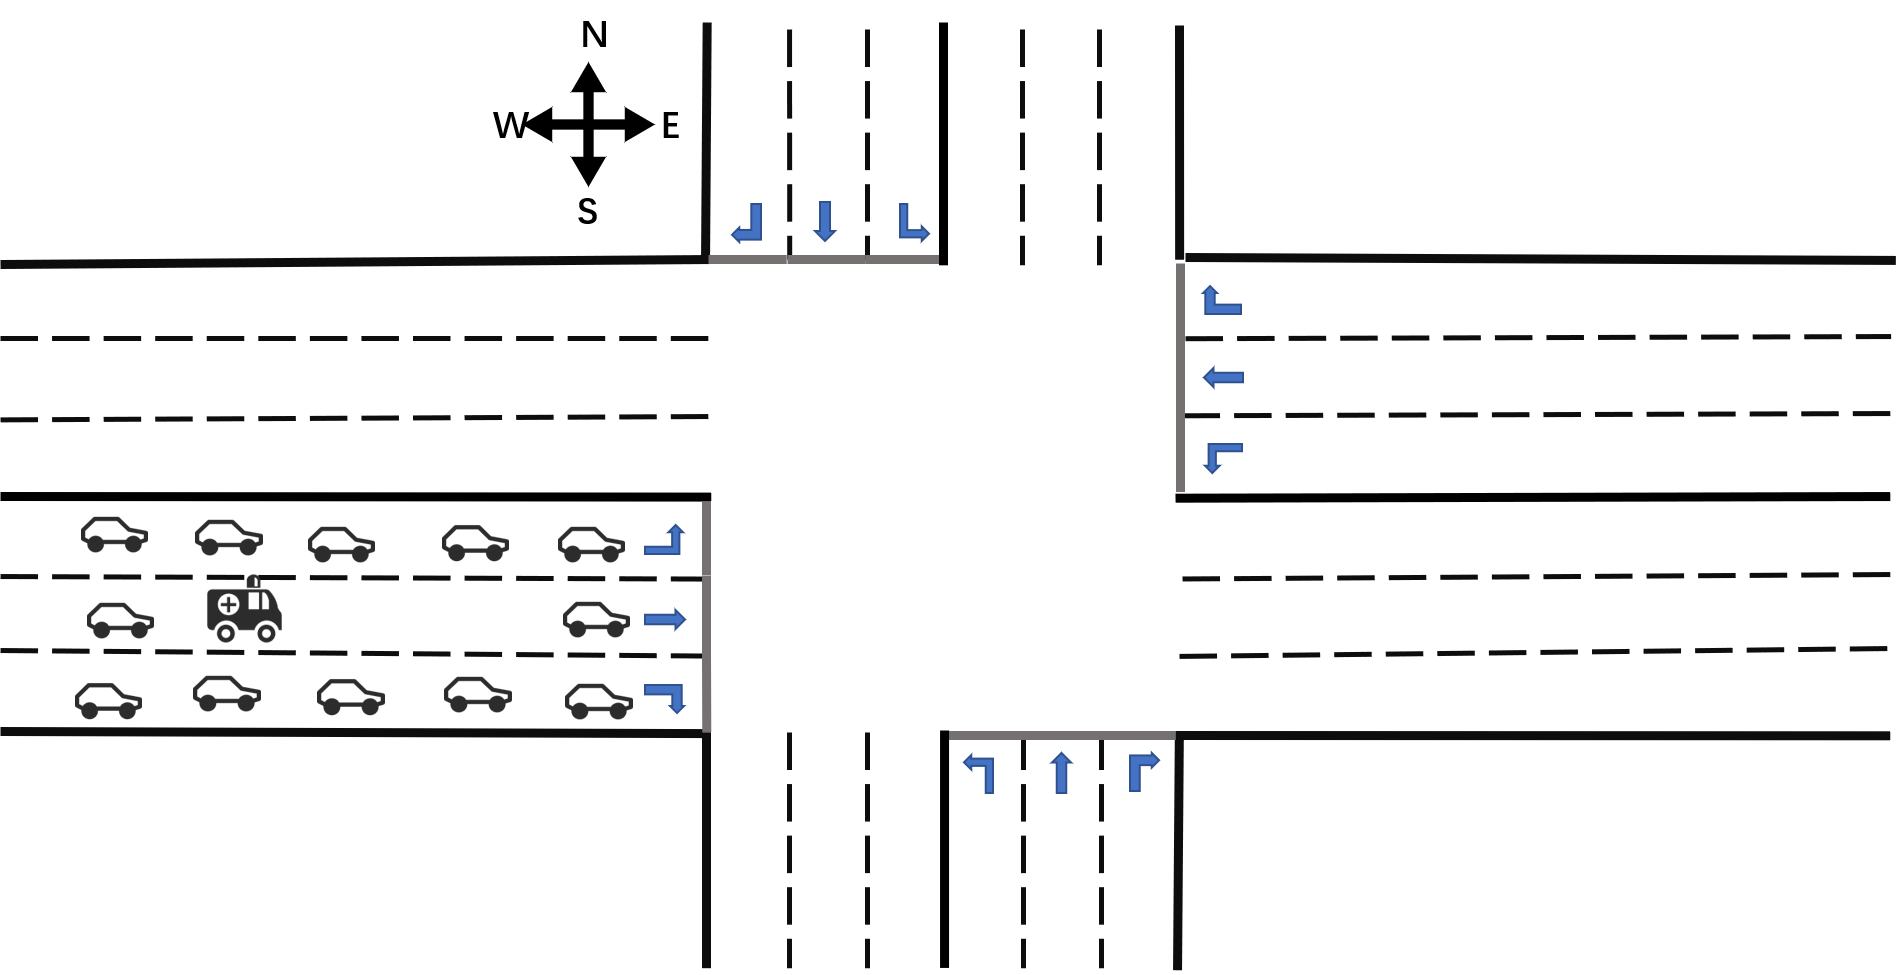
\includegraphics[width=\textwidth]{figures/tl_reduce.png}
	\caption{采取降低道路饱和度信号控制算法,应急车辆到达交叉口时道路情形图}
	\label{fig:tl_reduce}
\end{figure}

\begin{figure}[H]
	\centering
	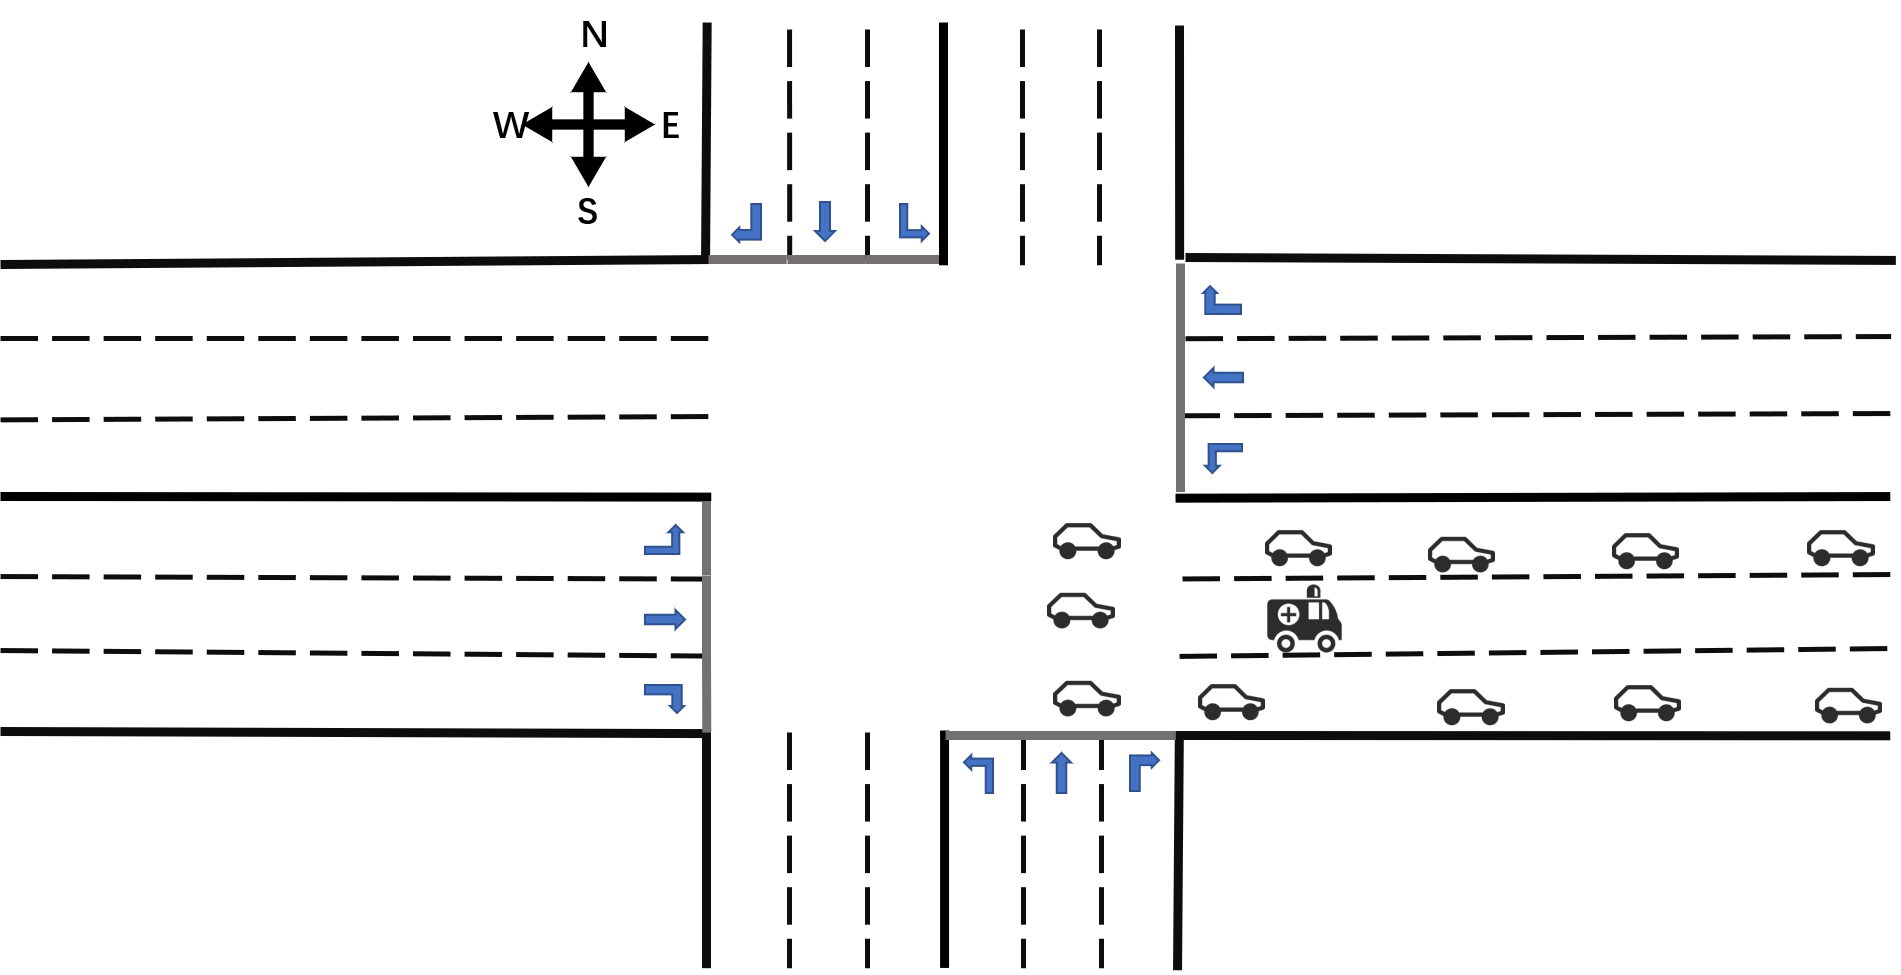
\includegraphics[width=\textwidth]{figures/tl_reduce_passed.png}
	\caption{采取降低道路饱和度信号控制算法,应急车辆通过交叉口后道路情形图}
	\label{fig:tl_reduce_passed}
\end{figure}

由上文可知,采取降低道路饱和度算法有三个突出优势:
\begin{enumerate}
	\item 智能体控制交通信号灯按需降低道路饱和度,使得距离应急车辆前方一定范围内的普通车辆有空间为应急车辆让行,应急车辆能够以更快的速度行驶,缩短了应急车辆的旅行时间;
	\item 由于饱和度降低以及普通车辆对应急车辆让行,应急车辆能以更快且更加稳定的速度向目的地行驶,使得速度偏差减小,预计到达时间的计算更加精确。
	\item 应急车辆在行驶的过程中,道路状况良好,交叉口排队车辆相对减少,提升了信号抢占阶段抢占方法的成功率,更容易体现面向应急车辆的“绿波带”效应;
	
\end{enumerate}

\subsection{降低道路饱和度程度模型构建}

本文中降低道路饱和度程度(The demand for reducing road saturation,简称DRRS)受到应急响应等级(Emergency Response Level, 简称ERL)、路段拥堵等级(Congestion Level of Road Section,简称CLRS)以及时间紧迫等级(Time Urgent Level, 简称TUL)三方面影响。
ERL是根据国家规定\cite{erl_2019}分为四级,CLRS根据标准\cite{GA_T_115_2020}分为四级,TUL表示应急车辆到达交叉口的时间紧迫程度,到达交叉口的时间越短,TUL越高。ERL越高,路段拥堵情况越严重,时间越紧迫,则应急车辆请求方向上的绿灯延长时间越长。此外本文不改变信号相位顺序,只增加相关相位的绿灯时间。

%关于紧急反应划分,根据国家大型突然性环境事故的紧急预案规定[64],根据各类突发公共事件按照其性质、严重程度、可控制和危害区域等因素,紧急反映评级分成非常严重(I级反应)、严重(II级反应)、严重(III级反应)、普通(IV级反应)等四级,如表4.1所示。

%对于应急响应等级,根据国家突发公共事件应急预案规定\cite{erl_2019},根据各类突发公共事件按照其性质、严重程度、可控性和影响范围等因素,应急响应等级分为特别重大(I级响应)、重大(II级响应)、较大(III级响应)、一般(IV级响应)四级,如表\ref{table:ERL}所示。

对于应急响应等级,根据国家突发公共事件应急预案规定\cite{erl_2019},ERL分为特别重大(I级响应)、重大(II级响应)、较大(III级响应)、一般(IV级响应)四级,如表\ref{table:ERL}所示。
\begin{table}[H]
	\centering
	\caption{突发事件应急响应等级}
	\label{table:ERL}
	\begin{tabular}{|c|c|}
		\hline
		应急响应等级(ERL) & 严重程度 \\ \hline
		I & 特别重大 \\ \hline
		II & 重大 \\ \hline
		III & 较大 \\ \hline
		IV & 一般 \\ \hline
	\end{tabular}
\end{table}

%根据标准GA/T 115-2020给出的城市主干路、次干路区间路段平均行程速度与交通拥堵度的关系\cite{GA_T_115_2020},如表\ref{table:GA}所示,将CLRS分为严重拥堵(IV级)、中度拥堵(III级)、轻度拥堵(II级)、畅通(I级)四级。本文给出了针对应急车辆的路段平均速度与交通拥堵关系,如表\ref{table:CLRS}所示。

%根据标准\cite{GA_T_115_2020},如表\ref{table:GA}所示,将CLRS分为严重拥堵(IV级)、中度拥堵(III级)、轻度拥堵(II级)、畅通(I级)四级。本文给出了针对应急车辆的路段平均速度与交通拥堵关系,如表\ref{table:CLRS}所示。

根据标准\cite{GA_T_115_2020},将CLRS分为严重拥堵(IV级)、中度拥堵(III级)、轻度拥堵(II级)、畅通(I级)四级。本文给出了针对应急车辆的路段平均速度与交通拥堵关系,如表\ref{table:CLRS}所示。

%\begin{table}[H]
%	\centering  % 显示位置为中间
%	\caption{城市主干路、次干路区间路段平均行程速度与交通拥堵度的关系\cite{GA_T_115_2020}}  % 表格标题
%	\label{table:GA}  % 用于索引表格的标签
%	%字母的个数对应列数,|代表分割线
%	% l代表左对齐,c代表居中,r代表右对齐
%	\begin{tabular}{|c|cccc|}  
%		\hline  
%		速度限制 & \multicolumn{4}{c}{ 平均行程车速(km/h)} \vline \\  % 表格中的内容,用&分开,\\表示下一行
%		\hline
%		80 & ${\geq{45}}$ & {[}30,45) & {[}20,30) & {[}0,20) \\
%		\hline
%		70 & ${\geq{40}}$ & {[}30,40) & {[}20,30) & {[}0,20) \\
%		\hline
%		60 & ${\geq{35}}$ & {[}30,35) & {[}20,30) & {[}0,20) \\
%		\hline
%		50 & ${\geq{30}}$ & {[}25,30) & {[}15,25) & {[}0,15) \\
%		\hline
%		40 & ${\geq{25}}$ & {[}20,25) & {[}15,20) & {[}0,15) \\
%		\hline
%		< 40 & {[}25,限速值) & {[}20,25) & {[}10,20) & {[}0,10) \\
%		\hline
%		拥堵程度 & 畅通 & 轻度拥堵 & 中度拥堵 & 严重拥堵 \\
%		\hline
%		路段拥堵等级 & IV级 & III级 & II级 & I级 \\
%		\hline
%	\end{tabular}
%\end{table}

\begin{table}[H]
	\centering  % 显示位置为中间
	\caption{针对应急车辆的城市路段平均速度与路段拥堵等级的关系}  % 表格标题
	\label{table:CLRS}  % 用于索引表格的标签
	%字母的个数对应列数,|代表分割线
	% l代表左对齐,c代表居中,r代表右对齐
	\begin{tabular}{|c|cccc|}  
		\hline  
		速度限制 & \multicolumn{4}{c}{ 平均行程车速(km/h)} \vline \\  % 表格中的内容,用&分开,\\表示下一行
		\hline
		80 & ${\geq{55}}$ & {[}40,55) & {[}30,40) & {[}0,30) \\ 
		\hline
		70 & ${\geq{50}}$ & {[}40,50) & {[}30,40) & {[}0,30) \\ 
		\hline
		60 & ${\geq{45}}$ & {[}40,45) & {[}30,40) & {[}0,30) \\ 
		\hline
		50 & ${\geq{40}}$ & {[}35,40) & {[}25,35) & {[}0,25) \\ 
		\hline
		< 40 & ${\geq{35}}$ & {[}30,35) & {[}25,30) & {[}0,25) \\ 
		\hline
		< 40 & {[}25,限速值) & {[}20,25) & {[}10,20) & {[}0,10) \\
		\hline
		拥堵程度 & 畅通 & 轻度拥堵 & 中度拥堵 & 严重拥堵 \\
		\hline
		路段拥堵等级(CLRS) & IV级 & III级 & II级 & I级 \\
		\hline
	\end{tabular}
\end{table}


对于TUL,根据预计到达时间分为严重紧急(III级)、比较紧急(II级)、一般紧急(I级)三级,如表\ref{table:TUL}所示。

\begin{table}[H]
	\centering
	\caption{预计到达时间与时间紧迫等级的关系}
	\label{table:TUL}
	\begin{tabular}{|c|c|c|}
		\hline
		${t_i}(min)$ & 时间紧迫等级(TUL) & 紧急程度 \\ \hline
		(0,5) & I & 非常紧急 \\ \hline
		(5,10) & II & 比较紧急 \\ \hline
		(10,30) & III & 一般紧急 \\ \hline
	\end{tabular}
\end{table}

%为了得到应急响应等级、路段拥堵等级以及时间紧迫等级对降低道路饱和度程度(DRRS)的影响程度,创建关于应急响应等级、路段拥堵等级以及时间紧迫等级相关的正互反矩阵,如表\ref{table:juzhen}所示,元素${i}$相对于元素${j}$的重要程度表示为${a_i^j}$。使用Santy1-9标度方法,判定各元素的重要程度,标度值及其含义如下表\ref{table:santy}所示。计算DRRS的目的是为了按需降低道路饱和度,当应急响应等级越高,则DRRS值越大,例如遇到特大火情,应急响应等级为I级,则应该牺牲交通成本来挽救生命和减少财产损失。道路饱和度与道路拥堵情况紧密相关,道路越拥堵,则DRRS值越大。时间紧迫等级越高,表示应急车辆预计到达时间越短,因此要尽快降低道路饱和度,反之,应急车辆还要等比较长的一段时间后才会到达交叉口,因此DRRS值可以小一些。

为了得到ERL、CLRS以及TUL对降低道路饱和度程度(DRRS)的影响程度,创建关于ERL、CLRS以及TUL相关的正互反矩阵,行元素${i}$相对于列元素${j}$的重要程度表示为${a_i^j}$。计算DRRS的目的是为了按需降低道路饱和度,当ERL越高,则目标相位延长的绿灯时间越长,例如遇到特大火情,ERL为I级,则应该牺牲交通成本来挽救生命和减少财产损失。道路饱和度与道路拥堵情况紧密相关,道路越拥堵,则则目标相位延长的绿灯时间越长。TUL越高,表示应急车辆预计到达时间越短,因此要尽快降低道路饱和度,反之,应急车辆还要等比较长的一段时间后才会到达交叉口,因此目标相位延长的绿灯时间可以短一些。


\begin{table}[H]
	\centering
	\caption{关于ERL、CLRS和TUL的正互反矩阵}
	\label{table:juzhen}
	\begin{tabular}{|c|c|c|c|}
		\hline
		指标 & \tabincell{c}{应急响应等级\\(ERL)}  & \tabincell{c}{路段拥堵等级\\(CLRS)} & \tabincell{c}{时间紧迫等级\\(TUL)}  \\ \hline
		应急响应等级(ERL) & 1 & 1/5 & 1/3 \\ \hline
		路段拥堵等级(CLRS) & 5 & 1 & 3 \\ \hline
		时间紧迫等级(TUL) & 3 & 1/3 & 1 \\ \hline
	\end{tabular}
\end{table}

%\begin{table}[H]
%	\centering
%	\caption{Santy1-9标度方法\ref{zhaojing_2003}}
%	\label{table:santy}
%	\begin{tabular}{|c|c|}
%		\hline
%		标度 & 含义\\
%		\hline
%		1 &	表示两个因素相比,同样重要 \\ \hline
%		3 &	表示两个因素相比,一个因素比另一个因素稍微重要 \\ \hline
%		5 &	表示两个因素相比,一个因素比另一个因素明显重要 \\ \hline
%		7 &	表示两个因素相比,一个因素比另一个因素强烈重要 \\ \hline
%		9 &	表示两个因素相比,一个因素比另一个因素极端重要 \\ \hline
%		2,4,6,8 &	上述两相邻判断的中值 \\ \hline
%		倒数 &	${j}$与${i}$比较的判断${a_j^i = \dfrac{1}{a_i^j}}$ \\ \hline
%	\end{tabular}
%\end{table}

各元素的权重关系可由使用本文信号控制方法所在地的实际情况进行评估,本文采用附录B中的调查问卷结果,得到如表\ref{table:juzhen}所示的正互反矩阵。其中CLRS比ERL明显重要,TUL比ERL稍微重要,CLRS比TUL稍微重要。最后经过归一化计算可得ERL的权重为0.1031,道路状况的权重为0.6053,预计到达时间的权重为0.2915。即可得降低道路饱和度迫切程度DRRS的评估模型为

\begin{equation}
	\label{equation:DRRS}
	DRRS={ERL}^{0.1031}\times{CLRS}^{0.6053}\times{TUL}^{0.2915} 
\end{equation}

%\subsection{面向单个应急车辆的降低道路饱和度方法}
\subsection{面向应急车辆的降低道路饱和度方法}

依据4级应急响应分级、4级路段拥堵等级和3级时间紧迫等级,DRRS一共有48种情况,使用K均值聚类算法将48种情况分为5个簇。最终分类结果如附录中表A所示,DRRS值越小,目标相位需要延长的时间就越长。

%\begin{figure}[ht]
%	\centering
%	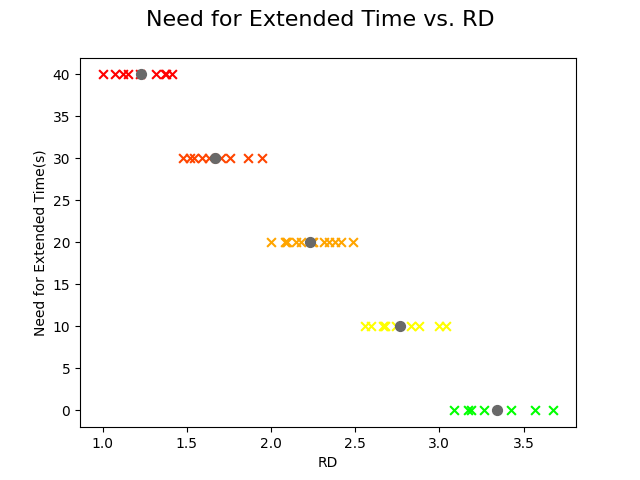
\includegraphics[width=\textwidth]{figures/kmeans.png}
%	\caption{DRRS值与延长目标相位时间的对应关系}
%	\label{fig:kmeans}
%\end{figure}


通过K均值聚类算法得出DRRS值所属的簇,每个簇对应不同的目标相位延长时间,如表\ref{table:extendtime}所示。但是随着时间的推移,ERL、CLRS以及TUL都有可能发生变化,ERL有可能升高也有可能降低,由于目标相位时间的延长,CLRS可能降低,也可能出现短时间内大量车辆涌入路段中导致CLRS升高,TUL随着时间升高,因此每秒钟都根据实际情况,计算DRRS值,如目标相位需要延长的时间发生了变化,则重新设置目标相位的时间,将目标相位的延长时间改为新的DRRS值所在簇对应的目标相位延长时间。例如,以ERL为Ⅰ级,CLRSⅠ级,TULⅡ级为例,DRRS值离1.2273的欧式距离最近,属于簇${c_1}$,应急车辆请求方向上的绿灯时间延长40s。经过一段时间后,ERL变为II级,CLRS降为II级,TUL升为I级,此时,DRRS值离质心1.6701最近,属于簇${c_2}$,目标相位绿灯时间延长40s改为延长30s。此外,在准备阶段的目标相位时长将一直作用到抢占状态结束。

\begin{table}[H]
	\centering
	\caption{目标相位延长时间参照表}
	\label{table:extendtime}
	\begin{tabular}{|c|c|c|c|}
		\hline
		簇 & 质心 & 簇内样本(ERL,CLRS,TUL) &  目标相位延长时间(s) \\
		\hline
		${c_1}$ & 1.2273 & (I,I,II) & 40 \\ \hline
		${c_2}$ & 1.6701 & (II,II,I) & 30 \\ \hline
		${c_3}$ & 2.2333 & (I,IV,I) & 20 \\ \hline
		${c_4}$ & 2.7658 & (IV,III,II) & 10 \\ \hline
		${c_5}$ & 3.3414 & (IV,IV,II) & 0 \\ \hline
	\end{tabular}
\end{table}


%\subsection{面向多个应急车辆的降低道路饱和度方法}
%当同一交叉口同时接受多个应急车辆的请求时,情况将会变得非常复杂,应急车辆可能来自同一方向,目标相位相同,也存在应急车辆来自不同方向,目标相位各不相同,或者多辆应急车辆有的来自相同方向,有的来自不同方向。对于不同的应急车辆,有不同的DRRS值。我们根据目标相位将应急车辆进行归类,目标相位相同的应急车辆归为同一类。同一类应急车辆DRRS值最大者为该目标方向的DRRS值。我们令${DRRS^k}$表示第${k}$相位的DRRS值,${DRRS_i^k}$表示目标相位为${k}$的第${i}$辆应急车辆的DRRS值。${DRRS^k}$的值为目标相位为${k}$的所有应急车辆中DRRS值的最大值。各相位时长为可以根据下式获得,${g^k}$为第${k}$相位的绿灯时长,${T}$为信号周期时长,${YR}$为信号相位切换时黄灯和全红的时长,${PN}$为该交叉口的相位个数。对于没有应急车辆请求的相位,按照ERL为IV级,道路拥堵等级按照道路本身的交通状况定级,事件紧迫等级为III级。假设十字交叉口有${PN}$个相位,因此各相位时长之和为周期减去${PN}$次切换的时长。各相位时长占比为该方向的DRRS值与各方向DRRS值之和的比值。

%\begin{equation}
%	\label{equation:gk}
%	g^k=\left(T-PN \times YR \right)\times\frac{DRRS^k}{\sum_{i=1}^{PN}{DRRS^i}}
%\end{equation}


\section{信号抢占方法}
本文为应急车辆提供了能够一路通行的快速通过“绿波带”方法,应急车辆总能够快速通过交叉口。降低道路饱和度能够让应急车辆以尽可能快的速度行驶,在接下来的文章中,本文将描述,怎样使得应急车辆无障碍通过路口,使应急车辆连续通过多个路口而无需停车。

%如何让应急车辆无障碍通过交叉口,使得应急车辆能够连续通过多个交叉口而无需停车。

\subsection{非侵入式信号抢占方法}
面向应急车辆的信号抢占策略已经被广泛研究,并且取得了不错的效果,闵万里等人\cite{min}通过修改信号周期与信号相位时长的方式让应急车辆到达时刻刚好落在目标相位,经落地实验表明,这种弹性信号抢占方案能够极大程度地降低应急车辆优先对整个交通造成的影响。因此,本文在此基础上,对他们的算法做了进一步的改进与创新,提出了一种基于多智能体的非侵入式信号抢占方法以体现面向应急车辆的“绿波”效应。

\begin{figure}[ht]
	\centering
	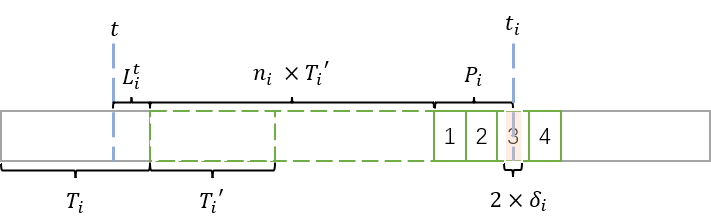
\includegraphics[width=\textwidth]{figures/non-invasive.png}
	\caption{非侵入式信号抢占方法}
	\label{fig:non-invasive}
\end{figure}

图\ref{fig:non-invasive}描述了非侵入式信号抢占方法的一个例子。交叉口${I_i}$的智能体${AGT_i}$在${t}$时刻接收到来自应急车辆的请求,根据式\ref{equation:t_i}计算出应急车辆预计到达交叉口${I_i}$的时间为${t_i}$,该方法尝试找到一个适用于交叉口${I_i}$交通信号灯的新周期${{T_i}^\prime}$(原周期为${T_i}$)和相位分配方案使得应急车辆到达交叉口${I_i}$的时间范围${[t_i-\delta_i, t_i+\delta_i]}$刚好落在目标相位中(本例中目标相位为相位3)。图中${L_i^t}$代表时刻${t}$到新周期${{T_i}^\prime}$第一次开始的时间间隔,${n_i}$表示信号灯从${t}$时刻到${t_i}$时间范围内完整新周期${{T_i}^\prime}$的个数,${n_i}$的计算公式为
\begin{equation}
	\label{equation:ni}
	n_i=\left\lfloor\frac{t_i-t-L_i^t}{{T_i}^\prime}\right\rfloor
\end{equation}
${P_i}$代表${n_i}$个新周期结束到${t_i}$的时间间隔,${P_i}$的计算公式为
\begin{equation}
	\label{equation:pi}
	P_i=t_i-t-L_i^t-n_i\times{{T_i}^\prime}
\end{equation}

本文结合实际情况,根据交叉口的排队车辆数,与实际通行率的比值,得出清空排队车辆所需的时间。清空应急车辆入口车道方向的排队车辆所需时间${Q_i}$计算为
\begin{equation}
	\label{equation:qi}
	Q_i=\frac{N_i^t}{S_i-Ai}
\end{equation}
式中${N_i^t}$代表${t}$时刻交叉口${I_i}$在应急车辆入口车道方向的排队车辆数目,${S_i}$则表示路口${I_i}$应急车辆入口车道方向的通行能力,代表了单位时间车辆通过该车道交通信号灯交叉口停车线的最大流量,${A_i}$为交叉口${I_i}$应急车辆入口车道方向的车辆到达率,${S_i}$与${A_i}$的差值为车道的实际通行率。

本文用代价时间${\Delta{w_i}}$表示交叉口清空应急车辆入口车道方向的排队车辆、确保应急车辆与普通车辆安全距离以及普通车辆为应急车辆让行需要的时间之和,${\Delta{w_i}}$表示为
\begin{equation}
	\label{equation:Delta_wi}
	\Delta{w_i}=\Delta_{i}\times(Q_i+(n_i+1) \times T_{lost} + SIT + YT )
\end{equation}
其中${Q_i}$为上文所述清空排队车辆所需时间,${T_{lost}}$为车辆启动损失时间,由于每一个周期内,应急车辆入口车道排队车辆都有启动损失时间,因此需要计算${n_i+1}$次车辆启动损失时间,${SIT}$(Safe Intrerval Time)为保证该交叉口行车安全的安全时间间隔,${YT}$(Yield Time)为交叉口普通车辆为应急车辆让行所需的时间,${\Delta_{i}}$代表在交叉口${I_i}$的应急车辆入口车道是否存在排队车辆,其值为
\begin{equation}
	\Delta_{i}=
	\begin{cases}
		0, & {N_i^t} = 0 \\
		1, & {N_i^t} > 0
	\end{cases}
	\label{equation:Delta_i}
\end{equation}
若应急车辆入口车道不存在排队车辆,即${N_i^t}$的值为0,则${\Delta_{i}}$的值0,若${N_i^t}$的值大于0,${\Delta_{i}}$的值为1。
%如式\ref{equation:Delta_wi}所示,我们用${\Delta{w_i}}$表示交叉口${I_i}$清空应急车辆入口车道排队车辆、确保应急车辆与普通车辆安全距离以及普通车辆为应急车辆让行需要的时间之和,

基于文献\cite{min}中QP二次规划问题(Quadratic programming,简称QP)来描述解决方案,定义了四种类型的变量:
\begin{enumerate}
	\item 输入:${PN}$代表周期中信号相位个数、${TP}$是目标相位、${g_i^k}$代表交叉口${I_i}$原本信号控制方案中第${k}$信号相位时长、${t}$代表当前时间、${t_i}$为应急车辆预计到达时间、${\delta_i}$代表应急车辆到达交叉口${I_i}$的时间偏差、${L_i^t}$代表应急车辆向智能体${AGT_i}$发出请求的时刻到原周期结束时刻的时间间隔、${{YR}_i}$代表交叉口${I_i}$信号相位切换期间的黄灯时间和全红时间之和;
	\item 超参数:${\beta}$代表目标函数中平衡总周期变化与单相时长变化的参数、${{T_i}^{min}}$和${T_i^{max}}$分别代表交叉口${I_i}$交通信号灯信号控制周期的上下界、${\tau_i^{min}}$和${\tau_i^{max}}$分别代表交叉口${I_i}$单相位时长的上下界;
	\item 输出:${g_i^{1^\prime}\ldots{g_i^{PN^\prime}}}$为优化后的各相位时长排列;
	\item 中间变量:${k}$代表信号相位序号,${i}$代表交叉口序号,${T_i}$和${{T_i}^\prime}$分别为交叉口${I_i}$当前周期时长与优化后的新周期时长、${n_i}$为第${i}$交叉口应急车辆预计到达时间之前的新周期个数。
\end{enumerate}

\newpage

\begin{equation}
	\label{qp:target}
	\min_{\left(T_{i}^{\prime}, g_{i}^{k^{\prime}}\right)}\left(\left(T_{i}{ }^{\prime}-T_{i}\right)^{2}+\beta \sum_{k=1}^{P N}\left(g_{i}^{k^{\prime}}-g_{i}^{k}\right)^{2}\right)
\end{equation}

\begin{subnumcases}
	{s.t.}
	T_{i}=\sum\limits_{k=1}^{PN} \left( g_{i}^{k} + YR_i \right), T_{i}^{\prime}=\sum\limits_{k=1}^{PN} \left( g_{i}^{k^{\prime}} + YR_i \right)\\ 
	%EAT = \sum\limits_{k=1}^{TP-1} \left( g_{i}^{k^{\prime}} + YR_i \right) \\
	%LAT = \sum\limits_{k=1}^{TP} \left( g_{i}^{k^{\prime}} + YR_i \right) - YR_i\\
	%EAT < P_{i} + \delta_{i} \leq LAT\\
	%EAT \leq P_{i} - \delta_{i} < LAT\\
	\sum\limits_{k=1}^{TP-1} \left( g_{i}^{k^{\prime}} + YR_i \right) < P_{i} + \delta_{i} \leq \sum\limits_{k=1}^{TP} \left( g_{i}^{k^{\prime}} + YR_i \right) - YR_i\\
	\sum\limits_{k=1}^{TP-1} \left( g_{i}^{k^{\prime}} + YR_i \right) \leq P_{i} - \delta_{i} < \sum\limits_{k=1}^{TP} \left( g_{i}^{k^{\prime}} + YR_i \right) - YR_i\\
	T_{i}^{min} \leq T_{i}^{\prime} \leq T_{i}^{max}\\
	\forall k \in PN, \tau_{i}^{min} \leq g_{i}^{k^{\prime}} \leq \tau_{i}^{max}\\
	n_{i} \times g_{i}^{TP^{\prime}} + P_{i} - \sum\limits_{k=1}^{TP-1} \left( g_{i}^{k^{\prime}} + YR_i \right) \geq \Delta w_{i}
\end{subnumcases}

二次规划的目的在于在满足式4.8a-4.8f的情况下,获取目标函数\ref{qp:target}的最优解。本文希望通过二次规划方法获得使得周期与信号相位时长变化最小的信号控制方案。目标函数的解需要满足式4.8a-4.8f的条件。式4.8a为原始周期与新周期时长的计算方式,式4.8b和式4.8c确保了预计到达时间落在目标相位上。式4.8d和4.8f分别代表信号周期时长与信号相位时长的时间限制,式4.8f确保了应急车辆到达时前方无排队车辆,且普通车辆能够为应急车辆让行,且保证了应急车辆通过交叉口后,普通车辆与应急车辆保持安全距离,应急车辆能够以更快的速度行驶。

本文对文献\cite{min}的改进如下:
\begin{enumerate}
	\item 将相位切换期间的黄灯时间和全红时间考虑在内,使得算法更加符合实际场景;
	\item 原文中排队车辆通过计算机视觉技术获取,将排队车辆长度除以清空排队车辆的速度(原文中为5m/s)获取清空排队车辆所需时。一方面受天气影响可能导致排队车辆计算不准确,另一方面没有考虑到${t}$到${t_i}$时间段内到达交叉口的排队车辆,因此本文通过传感器计算排队车辆数,并将${t}$到${t_i}$时间段内到达目标相位绿灯方向的排队车辆考虑在内,再结合车道通行能力与到达率更加精准地计算清空排队车辆所需的时间,本文计算清空排队车辆的方法更加科学合理;
\end{enumerate}

由于信号相位时长受到${\tau_i^{min}}$和${\tau_i^{max}}$的限制,信号周期受到${T^{min}}$和${T^{max}}$限制,对于预计到达时间较短的应急车辆,例如消防站附近的交叉口,智能体来不及为应急车辆规划出可行的非侵入式信号抢占方案,故本文提出了一种侵入式信号抢占方法,以弥补该算法的不足。

\subsection{侵入式信号抢占方法}
当非侵入式抢占方法无法得出可行解时,采取侵入式信号抢占方法。图\ref{fig:invasive}为侵入式抢占示意图,该方法在预计到达时间${t_i}$之前清空应急车辆前方排队车辆,保证普通车辆能够为应急车辆让行,以及保证应急车辆与普通车辆之间保持安全距离。

\begin{figure}[ht]
	\centering
	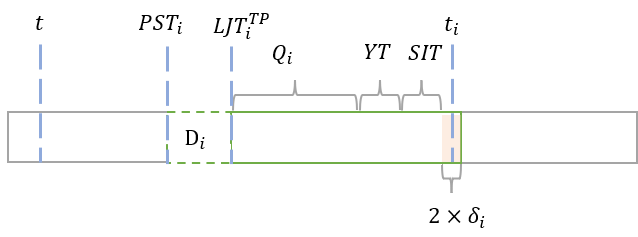
\includegraphics[width=\textwidth]{figures/invasive.png}
	\caption{侵入式信号抢占方法}
	\label{fig:invasive}
\end{figure}

图中${{LJT}_i^{TP}}$表示交叉口${I_i}$的交通信号灯最迟跳转到目标相位${TP}$的时刻,其值为
\begin{equation}
	\label{equation:D_i}
	{LJT}_i^{TP}=t_i-\delta_i\ -SIT-YT-Q_i
\end{equation}
其中${\delta_i}$代表应急车辆到达交叉口${I_i}$的时间偏差,根据式\ref{equation:delta_i}计算其值。${SIT}$(Safe Intrerval Time)为保证该交叉口行车安全的安全时间间隔。${YT}$(Yield Time)为交叉口普通车辆为应急车辆让行所需的时间。${Q_i}$为清空应急车辆入口车道方向的排队车辆所需时间,可根据式\ref{equation:qi}计算。信号灯最迟在${{LJT}_i^{TP}}$时刻跳转到目标相位,能够确保在预计到达时间之前能够清空排队车辆,并保证应急车辆与普通车辆之间保持安全距离,且保证了普通车辆能够为应急车辆让行。若信号灯跳转时刻大于${{LJT}_i^{TP}}$,则应急车辆入口车道的普通车辆无法为应急车辆让行,甚至无法清空排队车辆。若信号灯跳转时刻小于${{LJT}_i^{TP}}$,可能导致道路清空很长一段时间后,应急车辆才到达交叉口,这样会造成时间的浪费,并对其他方向的普通车辆造成影响。因此${{LJT}_i^{TP}}$必须保证在预计到达时间之前清空排队车辆,并保证应急车辆与普通车辆之间保持安全距离,以及保证普通车辆能够为应急车辆让行。


图中${PST_i}$为${{LJT}_i^{TP}}$在原信号控制策略中所处相位开始时刻。${D_i}$的值为
\begin{equation}
	\label{equation:D_i}
	D_i={LJT}_i^{TP}-PST_i
\end{equation}
表示若信号灯在${{LJT}_i^o}$时刻跳转到目标相位,被抢占相位持续的时间,其值为${{LJT}_i^o}$与被抢占相位开始时刻${{PST}_i^p}$的差值。

如图\ref{fig:jump_time}所示,计算出${{LJT}_i^{TP}}$和${D_i}$之后,需要根据${{LJT}_i^{TP}}$在原信号控制策略中所处相位是否为目标相位以及${D_i}$判断信号灯跳转的时刻。令${{Jump}_i^{TP}}$为交叉口${I_i}$智能体${AGT_i}$控制交通信号灯跳转到目标相位${TP}$的时刻,若${{LJT}_i^{TP}}$落在目标相位上,信号灯无需做多余的信号抢占,${{Jump}_i^{TP}}$的值为${PST_i}$。当${{LJT}_i^{TP}}$不在目标相位上,则${{Jump}_i^{TP}}$的值计算为
\begin{equation}
	Jump_{i}^{TP}=
	\begin{cases}
		PST_{i}, & D_{i}<G_{minS} \\
		LJT_{i}^{TP}, & D_{i}\geqslant G_{minS}
	\end{cases}
	\label{equation:jump}
\end{equation}
根据${D_i}$的值确定${{Jump}_i^{TP}}$,为保证行车安全,信号相位的持续时间不得小于保证行车安全的最短绿灯时间${G_{minS}}$,即当${D_i<G_{minS}}$时,${{Jump}_i^{TP}}$的值为${PST_i}$,否则${{Jump}_i^{TP}}$的值为最迟跳转时间${{LJT}_i^{TP}}$。侵入式抢占算法如算法\ref{alg:qinrushi}所示。

\begin{figure}[ht]
	\centering
	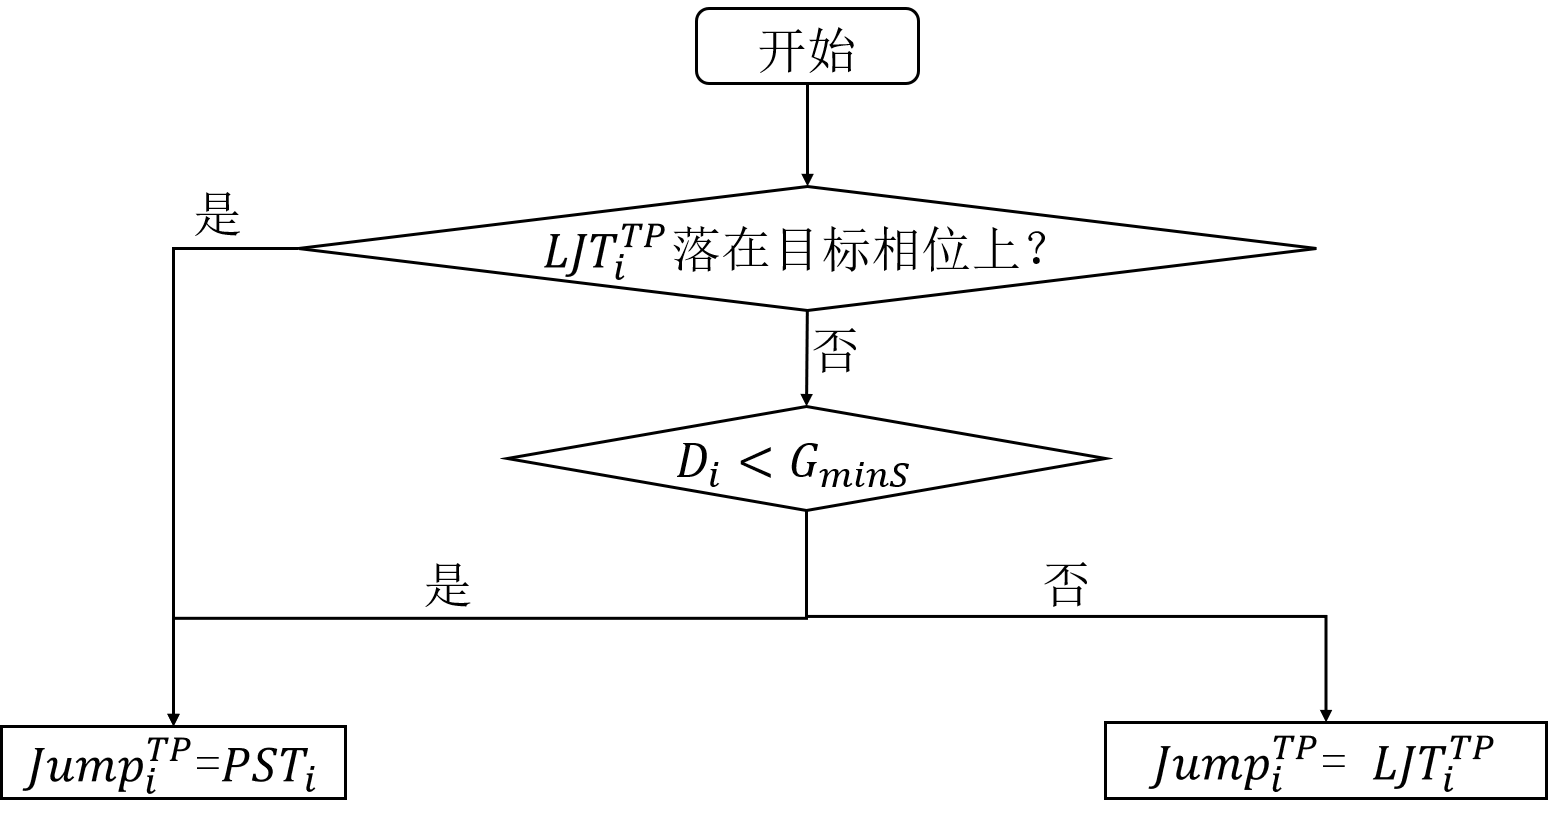
\includegraphics[width=\textwidth]{figures/jump_time.png}
	\caption{信号跳转的时刻}
	\label{fig:jump_time}
\end{figure}WW

\begin{algorithm}[!ht]
	\renewcommand{\algorithmicrequire}{\textbf{Input:}}
	\renewcommand{\algorithmicensure}{\textbf{Output:}}
	\caption{侵入式信号抢占算法}
	\label{alg:qinrushi}
	\begin{algorithmic}[1]
		\REQUIRE ${t_i}$, ${\delta_i}$, ${SIT}$, ${YT}$, ${Q_i}$  % input
		\ENSURE ${Jump_i^{TP}}$ % output
		
		\STATE ${{LJT}_i^{TP}=t_i-\delta_i\ -SIT-YT-Q_i}$
		\STATE ${D_i={LJT}_i^{TP}-PST_i}$
		
		\IF {${{LJT}_i^{TP}}$在目标相位上 or ${D_i < G_{minS}}$}
		\STATE ${Jump_i^{TP} = PST_i}$
		\ELSE
		\STATE  ${Jump_i^{TP} = LJT_i^{TP}}$
		\ENDIF
		
	\end{algorithmic}
\end{algorithm}


最终,信号灯在${{Jump}_i^{TP}}$跳转到目标相位,当应急车辆通过交叉口后,信号灯由信号抢占阶段进入恢复交通流阶段。


\newpage

\section{恢复交通流}
恢复阶段起始于应急车辆通过交叉口,然后以进入未请求阶段结束。该阶段能够让交叉口各方向车道排队车辆数尽可能恢复原貌,并且能够让信号控制方法恢复到信号抢占之前的初始信号控制方法。为达到恢复交通流的目的,本文使得交叉口各方向车道车辆排队数小于等于未请求状态下的平均排队车辆数${AVE_i^k}$。

当交通信号灯在某一信号相位下,将消散该信号相位绿灯方向的排队车辆,以图\ref{fig:intersection_phase}中图(1)为例,当交通信号灯处于该相位时,由西到东与由东到西两条车道上的车辆都会消散,这里以直行为例,先不考虑右转的情况。恢复交通流阶段需要将两条车道排队车辆数都恢复到没有应急车辆请求状态下的平均排队车辆数,因此仅需要考虑排队车辆数更多的车道即可,当信号相位时长能够满足将该车道排队车辆数疏散到小于等于没有应急车辆请求的平均排队车辆数,那么排队车辆数少的车道也能实现。

以图\ref{fig:ave_i_k}为例,假设样例中的交叉口为第1个交叉口,使得${N_i^k}$为恢复阶段开始时交叉口${I_i}$交通信号灯${k}$相位绿灯方向排队车辆数较大一边车道聚集的排队车辆数。例如,${N_1^1}$表示恢复阶段开始时交叉口1的交通信号灯在第1相位,即东西方向直行及右转相位时,绿灯方向排队车辆数较大一边的排队车辆数目。由图可得,东西方向直行及右转相位需要至少清除5辆车,东西方左转相位的需要至少清除4辆车,南北方向直行及右转相位的需要至少清除2辆车,南北左转相位的需要至少清除2辆车,因此有${N_1^1}=5$、${N_1^2}=4$、${N_1^3}=2$和${N_1^4}=2$。

\begin{figure}[H]
	\centering
	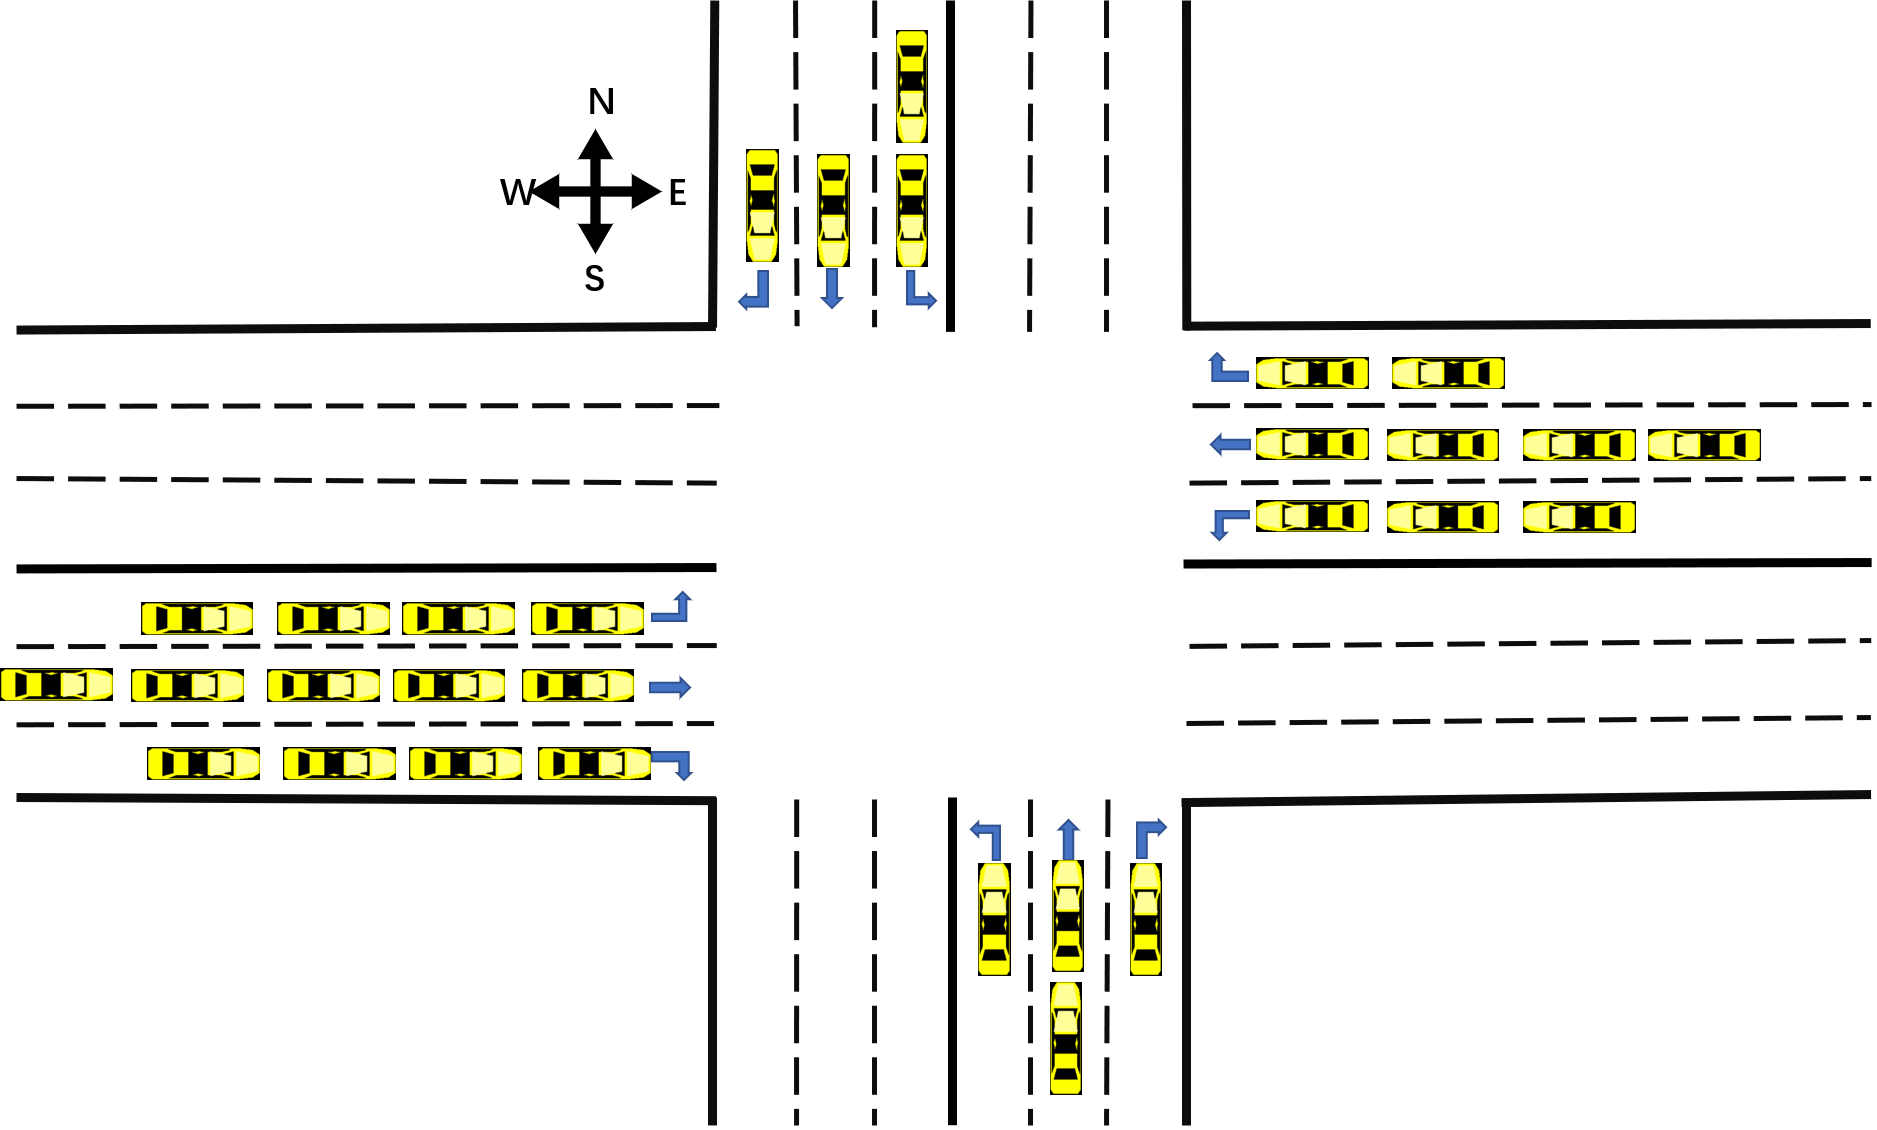
\includegraphics[width=\textwidth]{figures/nik.png}
	\caption{交叉口样例}
	\label{fig:ave_i_k}
\end{figure}

为使得交叉口各方向车辆排队数小于等于没有应急车辆请求状态下的平均排队车辆数。本文将该解决方案公式化为线性规划问题(Linear Problem,简称LP),表示为

\begin{equation}
	\min_{x_{i}^{k}}\sum_{k=1}^{PN}x_{i}^{k}
	\label{restoration_suanfa}
\end{equation}
\begin{subnumcases}
	{s.t.}
	\forall k \in PN, & ${\tau_{i}^{min} \leq x_{i}^{k} \leq \tau_{i}^{max}}$ \\
	\forall k \in PN, & ${EQN_i^k = N_{i}^{k} + A_{i}^{k} \times \sum\limits_{j=1}^{PN} x_{i}^{j}}$ \\
	\forall k \in PN, & ${VC_i^k = x_{i}^{k} \times S_{i}^{k}}$ \\
	\forall k \in PN, & ${EQN_i^k - VC_i^k \leq AVE_{i}^{k}}$
	\label{restoration_st}
\end{subnumcases}
其中,${x_i^k}$表示交叉口${I_i}$的交通信号灯在恢复阶段第${k}$相位的时长,式\ref{restoration_suanfa}为目标函数,目的是让过渡阶段各相位绿灯时长之和最短,这样就能够在最短的时间内将交通流恢复到没有应急车辆请求状态。在使得各相位绿灯时长之和最短的同时,需要满足式4.13a-4.13d。式4.13a确保了各相位绿灯时间在最小绿灯时间${{\tau_i}^{min}}$和最大绿灯时间${{\tau_i}^{max}}$之间。式4.13b中${EQN_i^k}$表示第${i}$个交叉口第${k}$相位预计排队车辆数,其值为${N_i^k}$与恢复周期内到达的排队车辆数之和,式中${A_i^k}$为交叉口${I_i}$第${k}$相位绿灯方向车道的到达率,${A_i^k\times\sum_{j=1}^{PN}\left(x_i^k+YR_i\right)}$为恢复阶段到达交叉口第${k}$相位绿灯方向车道的排队车辆数。公式4.13c中${VC_i^k}$表示第${i}$个交叉口第${k}$相位在该相位时间内能够清除的排队车辆数,${S_i^k}$为交叉口${I_i}$交通信号灯${k}$相位绿灯方向车道的饱和流率,${x_i^k \times S_i^k}$为${x_i^k}$时间内疏通的排队车辆数。式4.13d中${EQN_i^k - VC_i^k}$为恢复阶段结束时,该车道的排队车辆数,其值应小于等于${AVE_i^k}$。

当应急车辆通过交叉口后,智能体通过恢复阶段信号控制算法设置交通信号灯各相位绿灯时长,待各相位结束,交通信号灯恢复到没有应急车辆请求下的信号控制方案。本文通过整个交通路网中的平均等待时间反映恢复阶段的效果。车辆等待时间一般表示车速低于或等于0.1m/s的时间,因此在本文中车辆等待时间为车辆等红灯的时间,以及道路拥挤或发生车祸情况下的车速低于或等于0.1m/s的时间,整个交通路网中的平均等待时间是整个交通路网中所有车辆的等待时间的平均。平均等待时间越小,表示本文恢复策略表现效果越好。这将在第5章的实验中详细分析。
%智能体使用恢复阶段信号控制方案控制交叉口交通信号灯,当恢复阶段结束时,智能体将交通信号灯的信号控制方案设置为没有应急车辆请求下的控制方案,恢复阶段结束。

\section{本章小结}
本章提出了一种面向应急车辆优先的“绿波带”信号配置策略,通过提前降低道路饱和度、为应急车辆提供信号抢占以及恢复整个交通流三个阶段保障应急车辆一路快速绿灯通行。第一阶段降低道路饱和度程度(DRRS)根据应急响应等级(ERL)、路段拥堵等级(CLRS)以及时间紧迫等级(TUL)得出目标相位绿灯延长时间。为确保应急车辆到达交叉口时能快速通过交叉口,第二阶段结合侵入式抢占方法与非侵入式抢占方法为应急车辆提供绿灯指引,使得应急车辆能够快速通过交叉口而不停止。第三阶段通过重新规划信号周期与交叉口各相位绿灯时间,调节交叉口各入口方向交通流量,降低应急车辆优先对整个交通造成的影响。
